\chapter{Experiences of Science Capital in University Science}

\section{Preamble}
The following chapter details the results of a set of nineteen interviews that were conducted with science students at the university of Auckland. I mirror the structure of the previous chapter, where I outline arguments for a conceptual model of how capital is accumulated by students as university. The current chapter, in addition to detailing the qualitative methodologies employed, will seek to add the colour of life experiences to my conceptual model. It is in this chapter where I seek more understanding of \textit{why} students do or do not choose to study science.

\subsection{Capital in the Field of University Science Education}



\subsection{Introduction}
The goal of the current chapter is to explore how the conceptual model outlined in Chapter 5 is experienced by students at the University of Auckland (UoA). More specifically, I seek to answer three specific research questions:
\begin{itemize}
    \item What forms of social capital are available to university science students? 
    \item How do students leverage social capital to gain advantage in the field of university science? 
    \item How does students' habitus contribute to the accumulation of capital?
\end{itemize}

I adopted a staggered research design, where the research process took place over three separate phases. As shown in Table \ref{tab:Phases}, the process began with four interviews with students in the science scholars programme (a programme for gifted science students) at the UoA. Based on preliminary data from these interviews and a questonnaire provided by the ASPIRES research group in the United Kingdom \citep{dewitt2011high}, a questionnaire was designed to assess the relationships between students' social capital, cultural capital, social location (gender, ethnicity, socio-economic status), and confidence in science. The questionnaire asked students to record factual information about themselves, and answer items regarding 5 latent constructs informed and adapted from the work of \cite{dewitt2011high}. The constructs included self-concept in science (Science Self-concept), experience of high school science teachers (Science Teachers), parental attitudes towards science (Science Parents), peer attitudes towards science (Science Peers), and access to science-related resources (Science Resources). Results of a Confirmatory Factor Analysis (CFA) provided support for these 5 factors ($\chi^{2} =$ 483.74, $\mathrm{df} =$ 179, p $<$ .001, CFI  $=$ 0.93, TLI  $=$ 0.91, RMSEA $=$ 0.05), while separate tests of showed adequate reliability of each construct (McDonald's $\omega$ 0.68 - 0.86). More detailed information regarding questionnaire design and quantitative results is available in Chapter 4. 
\begin{table}[ht]
\begin{tabular}{c|c|l}
                      
Phase  & Year & Purpose    \\ \hline
1   & 2018  & Interviews with 4 high achieving science students at UoA.     \\
& & Results of these interviews were used to inform questionnaire design. \\ \hline
2  & 2018-2019 & Questionnaire design and administration to science students at UoA.  \\
& & Questionnaire analysis conducted (see Chapter 4)\\ \hline
3 & 2019 & Main interviews conducted with 15 students. \\
& & These were selectively sampled from the questionnaire. \\ \hline
\end{tabular}
\caption{\label{tab:Phases} The timeline of the qualitative research process. Preliminary interviews with four high achieving science students informed the design of questionnaire, which was administered to science students at UoA in early 2019. Fifteen students were then purposefully sampled for interviews based on questionnaire responses.}
\end{table}

The current study draws from the pool of questionnaire respondents. The staggered research design has been used in previous research to investigate student experiences in STEM to great effect \citep{grossman2014perceived,russell2011factors}. Whereas previous research has focused on random sampling \cite{russell2011factors} or purposeful sampling to achieve a balance of gender or ethnicity in interviews \citep{grossman2014perceived}, the current study seeks to take a more intersectional methodological approach by including domain-specific indicators of social class as well as self-report measures of gender and ethnicity in the decision making process. As shown in \ref{fig:ScienceFactors_C6}, students were purposefully sampled from a range of different social locations, with the aim of representing a range of student experiences. Through interviews with these students, it may be possible to untangle some of the complexities that surround the impact of parents, peers, and resources on experiences of university science education. The following section will outline the methods used in the interview phases in more detail.

\begin{figure}[ht]
\centering
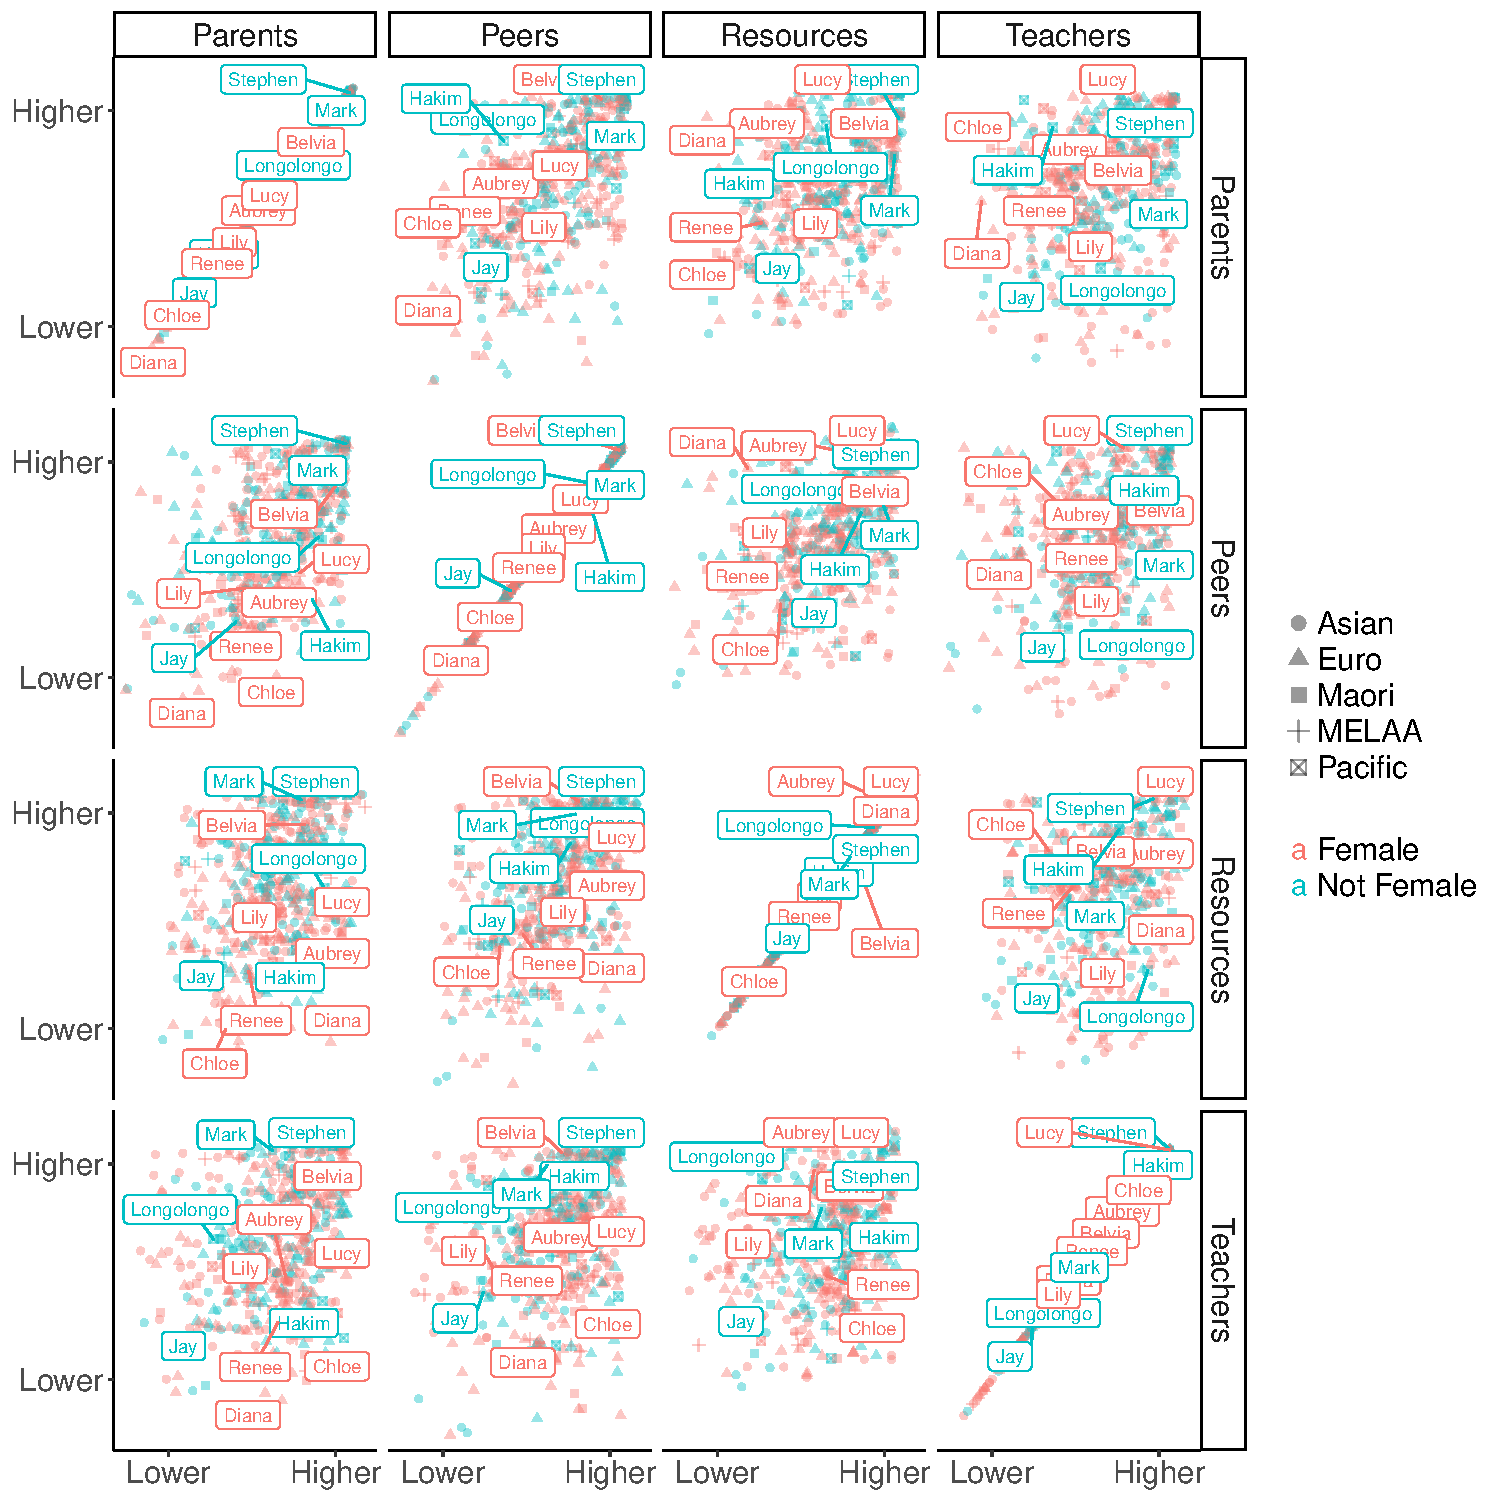
\includegraphics[width=\textwidth]{C6 - Experiences of Science Capital/ScienceFactors_FacetPlot.pdf}
\caption{\label{fig:ScienceFactors_C6}\textbf{Sampling Strategy}. The above plot shows the methods used to sample students when arranging interviews. I aimed to interview students with a range of different backgrounds with regards to forms of science capital. Axes indicate the students' level of a particular form of capital, including Science Parents, Science Peers, Science Resources, and Science Teachers. The locations of 12 of the 19 interviewee participants are highlighted by their pseudonym. The four participants interviewed at phase 1 are not included, while three interview participants from phase 3 were excluded from factor analysis due to having too much missing data in the questionnaire (see Turnbull (in review) for more details). Individual data points are also coloured and shaped at the intersection of identified gender and ethnicity. In this case, ethnicity is coded according to prioritised ethnicity, where students who identified with multiple ethnicities were first coded as M\={a}ori, then Pasifika, then Asian, then European (following guidelines set out by Statistics New Zealand). I only use the prioritised ethnicity for ease of plotting and not for any analysis. Gender in this case refers to whether the individual self-identified as female or not. }
\end{figure}

\section{Methods}

\subsection{Context}
The current study discusses data from nineteen semi-structured interviews conducted with students enrolled in STEM subjects at the University of Auckland (UoA). Four students were invited to interview based on their participation in the science scholars programme at the UoA, and fifteen students were purposefully sampled from the pool of questionnaire respondents. Given the goal of these interviews is to reveal variation in the students experiences in science, rather than to discuss the properties of a `sample', it can be argued that a sample size of 19 participants is sufficient \cite{berglund2006students}. For participants drawn from the questionnaire, sampling was prioritised based on the constructs of capital measured in the questionnaire (Figure \ref{fig:ScienceFactors}), and also according to whether they identified as a member of an underrepresented social group in science. The purposeful sampling was a deliberate choice informed by research on intersectionality. As outlined by \cite{duran2019using}: ``Even if multiple marginalized demographics are not the subject, they must always be centered.'' The social groups I intentionally sampled were thus as follows:
\begin{itemize}
    \item Individuals with lower levels of science related capital. This judgement was made based on students reported scores on the teachers and peers value of science constructs, which were found to be the most important predictors of self-concept in science in Chapter 4.  I also took into account other indicators of science-related capital, such number of books at home growing up and access to science related activities.
    \item Individuals with parents who do not value science, or who do not talk about science often. Even though parents value of science was not a significant predictor of science self-concept in Chapter 4, I expected it to still play a major role in participants' development of habitus in science. 
    \item First generation to university students. 
    \item M\={a}ori and Pasifika students. While research has explored factors relating to success at university in general for students identifying as M\={a}ori and/or Pasifika \citep{mayeda2014you}, there is a need for research that seeks to present their experiences in science specifically. 
    \item Female students in physics and computer science. Through interviews with these students we may begin to describe why we see certain trends in student enrolments, such as those described in Chapters 2 and 3.
\end{itemize}
While the above criteria represent the students of specific interest, the students interviewed represented a range of social backgrounds, with some students representing multiple criteria and some not representing any. It is also important to note that the categories employed are simplistic and do not encompass a range of other important characteristics (such as religion or ableness), or indeed the complexity of belonging to multiple groups. While much research of marginalised groups in science is grounded in deficit-theorising (why do students drop out?), the current study attempts to adopt an asset-based framework (why do students succeed?). This framing is prefaced by the acknowledgment that while resilience should be celebrated, it should not be necessary. Participant characteristics are summarised as in Table \ref{tab:Demographics} and participant summaries are also available as supporting information. 


\begin{table}[ht]
\begin{tabular}{cc|c}
                       &                        & Count \\ \hline
Gender                 & Male                   & 7     \\
                       & Female                 & 8     \\ \hline
Ethnicity              & Asian                  & 3     \\
                       & M\={a}ori                  & 7     \\
                       & Pasifika               & 3     \\
                       & Pakeha/European        & 9     \\ \hline
University Generations & First Generation       & 7     \\
                       & Sibling                & 2     \\
                       & Parent                 & 4     \\
                       & Grandparent and Parent & 2     \\ \hline
Subject Disciplines    & Biology                & 8     \\
                       & Chemistry              & 7     \\
                       & Computer Science       & 6     \\
                       & Mathematics            & 3     \\
                       & Physics                & 7     \\
                       & Psychology             & 3     \\
                       & Statistics             & 4     \\ \hline
Self-concept          & Higher                   & 7     \\
                       & Lower                    & 5     \\ \hline
Science Parents        & Higher                   & 8     \\
                       & Lower                    & 4     \\ \hline
Science Teachers       & Higher                   & 7     \\
                       & Lower                    & 5     \\ \hline
Science Peers          & Higher                   & 7     \\
                       & Lower                    & 5     \\ \hline
Science Resources      & Higher                   & 8     \\
                       & Lower                    & 4    
\end{tabular}
\caption{\label{tab:Demographics} A table summarising the characteristics of the individuals who participated in interviews following completion of the questionnaire. Aggregated group counts are provided to help preserve anonymity. Participants may have identified with multiple ethnicities or be enrolled in multiple subject disciplines, which means that these counts do not sum to fifteen. Three students who participated in interviews did not provide enough information on construct items to have scores on self-concept and capital scales attributed to them. Information is not presented for the four students who completed the first interview phase of the study, prior to administration of the questionnaire.}
\end{table}

\subsection{Qualitative approach and research paradigm}
Interview questions were based on the items presented to participants in the questionnaire. These questions reflect a deductive approach, where previously established theory guides questions. This process was conducted explicitly by using the participants' questionnaire responses as an object for discussion. For example: 
\blockquote{On this section: my friends see me as a science person. You scored quite highly - how do you feel about that?} While interviews were directed by participants' questionnaire responses, they were also semi-structured. This means that participants were invited to lead discussion and talk about what they felt was important. As M\={a}ori were invited to be interviewed, this inductive approach was informed by Kaupapa-M\={a}ori-Consistent (KMC) practices. KMC practice requires research concerning M\={a}ori to be conducted with, and not on, M\={a}ori \citep{walker2006exploration}. My attempts to adhere to KMC practices meant that the conceptualisation and operationalisation of research procedures were also discussed with M\={a}ori representatives, and that participants were offered transcripts of interviews and manuscript drafts, and invited to remove, edit, and add responses after the interview.  

An inductive approach to thematic analysis was used to analyse the interview transcripts, following the general guidelines set out by \cite{Braun_2006}. Interviews were coded in accordance to the the three established research questions:  what forms of social capital are available to university students? How do students leverage social capital to gain advantage in the field of university science? And finally, how does students' habitus contribute to the accumulation of capital? Themes were then established and developed into the conceptual model outlined in Chapter 5 to aid in answering these questions. Bourdieu's sociological theory was employed as a conceptual ``toolbox'', drawing primarily on his concepts of social capital, habitus, field and doxa. The conceptual model (Figure \ref{fig:HabitusSocCap_TheoreticalModel_C6}) provides a lens to explore how social capital impacts on habitus, and how habitus then influences future capital accumulation. 

\begin{figure}[ht]
\centering
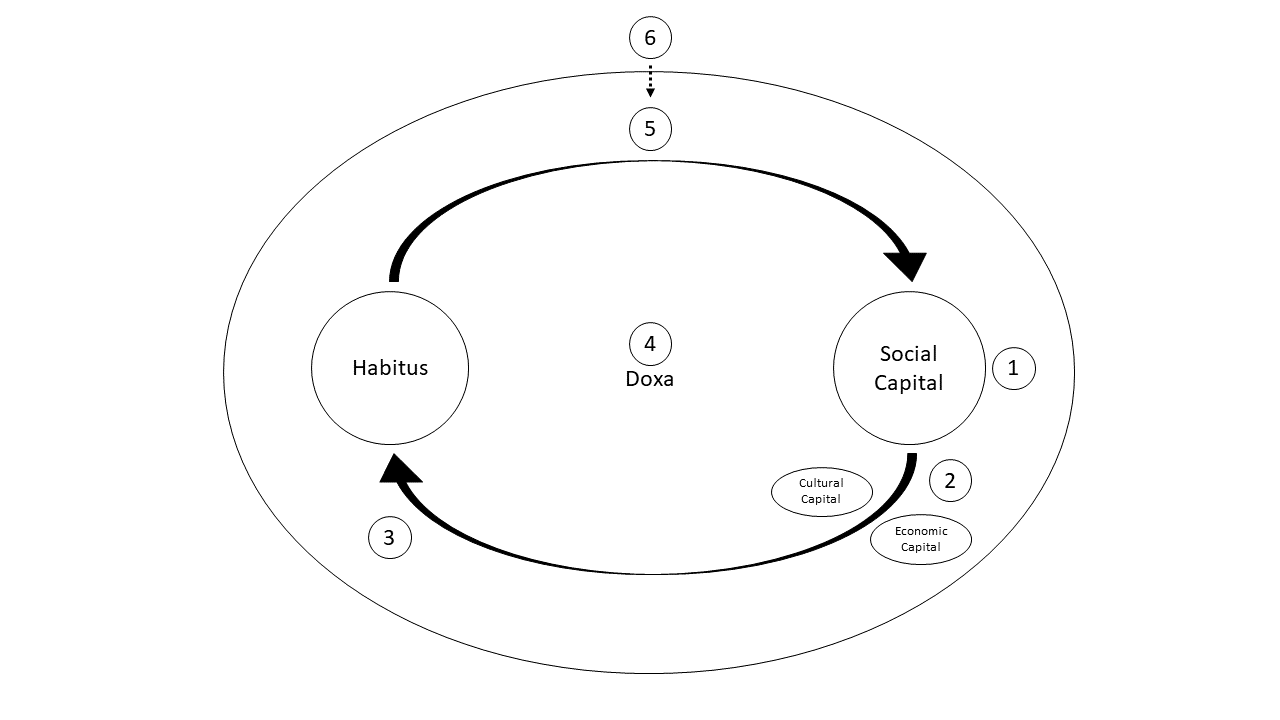
\includegraphics[width=\textwidth]{C5 - Understanding Capital Accumulation/HabitusSocCap_TheoreticalModel.png}
\caption{\label{fig:HabitusSocCap_TheoreticalModel_C6}\textbf{Conceptual Model}. The conceptual model used to understand individual practices in the field of science education. The model, informed by the experiences of participants in the current study, expands on the interaction between habitus and capital originally illustrated by \cite{Bourdieu1984}. The model provides a step by step description of how social capital translates into habitus transformation, and how habitus generates future capital accumulation. Step 1 refers to the initial availability of social capital for an individual. Step 2 refers to the value gained through leveraging social capital into forms of economic and cultural capital. Step 3 refers to how social capital is internalised by the individual. Step 4 refers to how habitus informs the acquisition of future social capital. 5 refers to factors outside of the individual that structure the field (by availability of capital and exchange value).}
\end{figure}

The following sections will describe the perceptions of participants, following the structure of the conceptual model outlined in Chapter 4. While much of my discussion simply describes the experiences that participants reported (semantic themes), the goal of my analysis is to be interpretative \citep{Braun_2006}. This means that I intend to go beneath the level of description and to place participants' experiences into the conceptual model, which I theorize shapes the experiences of participants. Prior research is referenced to support my interpretations. 

\section{Social Capital in the Field of University Science (Step 1)}
This section discusses the availability of social relationships that participants had in the field of university science (Step 1 in Figure \ref{fig:HabitusSocCap_TheoreticalModel_C6}). These relationships are categorised into three key groups, social capital through family connections, social capital through lecturers, and social capital through peers. 

\subsection{Family, Whanau, and Significant Others}
Students' upbringing within the their family and whanau played an important role in students experiences of university science. The M\={a}ori term \textit{whanau} refers to extended family or a community of related families, and therefore this theme refers to the social capital student's held via their parents and siblings, but also through aunties, uncles, and grandparents. Access to social capital through family differed across participants' experiences. Some participants came from highly academic families with science backgrounds, others had whanau with little experience of science education.

Some participants had family that were interested in science and were available to  talk about it. 

In some cases, participants found they needed to step away from family, whanau, or significant others who did not value science education in order to aid their educational journey. Renee identified the moment that she left a controlling partner as a key moment in their pursuit of education: \blockquote{It is like when you hold a spring down and it has got so much potential and then you let it go and it is like fuck yeah, do you know what I mean, like that was me leaving that person and being like yeah.}. Leaving a relationship where values regarding education are not shared gave Renee a renewed sense of potential. Hakeem, who argued that ``the priorities are very different for Islanders'' found that moving into his own space allowed him to focus more on his education: \blockquote{...just having that kind of space and gap from your family it was really huge for me.} Previous research suggests that family responsibilities place more demands on Pasifika and M\={a}ori students \citep{zepke2011non}. In a study of post graduate Pasifika university students, \cite{theodore2018pacific} found that family responsibilities were the most commonly cited factor that hindered qualification completion. With that being said, the support of family was the most cited source of help for students, a finding that is reflected in the experiences of participants in the current study. Participants acknowledged the importance of having family support: \blockquote{} Attending a university in a different geographical location to family could decrease the availability of this form of social capital: ``''


\subsection{Educators}
The relationships participants shared with their high school teachers, university tutors and lecturers were highly influential in shaping students experiences of university study. The availability of lecturers as sources of social capital was informed by participants' knowledge of how to approach them, and participants' perception of how approachable they were. 

Following the transition to university, some participants were aware that the rules may be different and that their may be different conventions to follow when communicating with lectures. Paul, a science scholar with mentors at university, did find it difficult to know what conventions to follow:
\blockquote{I haven't emailed anyone, I think about it but again I don’t know how I am supposed to approach anyone... I'm never really sure how things work in a university environment, how polite can you be, how do you contact these people in the first place}. Participants were most likely to develop relationships with their lecturers when they were perceived as kind, happy and enthusiastic. 

In other cases, participants felt that their lecturers were not available or accessible, with this being informed both explicitly and implicitly. some participants felt that their lecturers were too intimidating or ``distant'' (Longolongo). Sometimes these feeling of intimidation were based on explicit past interactions: ``[the lecturer] definitely did not care because he was like so ruthless. He was like no that is a dumb question.'' (Belivia).



\subsection{Peers}
Participants' recalled different types of social relationships with peers. Some participants we able to talk about science with their peers, while for others conversations would focus on other aspects of their lives. 

While some participants entered into university study with a cohort of students from the same school, other participants entered university with limited peer networks.  


\section{Leveraging Social Capital (Step 2)}
The value of social capital is derived from the economic and cultural capital that can be mobilised through the connection. These resources may provide students with advantages in supporting their learning and providing student access to information about the field. 

\subsection{Family, Whanau, and Significant Others}
Participants who did not have parents who went to university had to find other sources of information on navigating university pathways. Participants were able to leverage family connections to get employment opportunities, but this was not possible if family connections were not there. Hakeem found attaining work hours for his engineering degree difficult, but observed that other students ``had connections with their family their dad was an engineer''. Having family, whanau, or significant others that were scientists provided participants with a flow of information about what the field was like. Regardless of education, having family talk about science could also help spark participants' interest. 

Some participants recalled their parents allowing them to find their own pathway: \blockquote{I think they have always kind of taken the stand that I can sort of dictate where my future goes.} (Lily). For these participants, parents provided everyday support and encouragement, with the main goal for their children to do something that makes them happy. Other participants recalled a more hands-on form of support, where parents would encourage them academically and set expectations for their education. This kind of behaviour can be defined as \textit{concerted cultivation} \citep{lareau2011unequal}, and it was a common experience for participants who had university educated parents. Concerted cultivation can be more implicit and subtle than overt sources of pressure from family. Chloe summarised this concept by referring to they way in which she had been ``groomed that you go to university''. Some participants outlined the ways in which parents kept tabs on their academic progress and advocated for them when they felt the school was not meeting expectations. For example, Jay recalled how his mother taught him mathematics at home when she felt that the school teaching him enough.

\subsection{Educators}
Connections with educators offered an important source of support for participants. They were able to answer student's questions on course content, provide advice on study techniques, and give ``insight'' (Susan) on academic pathways. ``he helps me with everything so him being really supportive and really kind it really helps me.'' (Belvia).

Participants who entered university with gaps in their knowledge may be less able to understand the content that is being taught. Students who feel a tacit ``distance'' from lecturers may also be less able to leverage value from the relationship. As described by Longolongo, ``you are not writing for yourself you are writing for them, for their perception''. Longolongo felt it would be better if their lecturer was ``on the same level'' or in the same ``mindset'' as him. 



\subsection{Peers}
For most participants, academic peers were a source of support. This support was utilised explicitly through advice seeking and direct help. Participants saw the benefit of having close peers who they were able to study with. Through their relationships with their friends and academic peers, participants were also able to gain more information on academic pathways, the support groups available to them at university, and what future careers looked like. For example, Mark recalled his resident advisor recommending that he attend lectures for more advanced courses to give him some idea of what the future could hold. Peers could also offer support in a tacit manner, by offering role models for learning, or through vicarious learning experiences (e.g., learning through the questions that peers asked). 

Beyond academic support, participants were grateful for friends that offered them a general, everyday support. Hakeem found that having  consistent For participants who did not have friends who pursued science at university, sharing that knowledge with them could be fulfilling and help ``grow your self-confidence'' (Renee).



\section{Internalising Social Capital (Step 3)}
The social capital that students accrue in university science not only provides access to resources, but it can also influences the way that students see themselves in the field. Capital, which determines students position in the field, is internalised by students via their habitus, which establishes the students disposition towards the field \cite{Bourdieu1992}. Students who hold high levels of social capital may feel an affinity with the field and see progression to university as a ``path already kind of drawn out'' (Chloe), ``inevitable'' (Susan), and those who identified as ``smart'' (Paul) or ``academic'' (Mark) felt like they almost had an obligation to study science. Those who have fewer connections may not feel like the belong, which may be manifested in feelings of not being ``smart enough'' (Patrick), questioning ``should I be here?'' (Renee), or not feeling ``good enough for that space.'' (Hakeem). These feelings can be conflicting, as Longolongo described: ``I feel like I belong in science but I haven’t convinced myself that I belong there''. When asked what it would take to convince Longolongo that he belonged in science, he responded ``I was going to say I need someone to convince me, but no I don’t think so. I think I just have to convince myself''. Longolongo's response brings to light a key aspect of habitus, that while relationships with others are important, we perceive that our convictions are self-directed. The following section expands on how of social relationships with family, educators, and peers are internalised and shape our perceptions of belonging.
 


\subsection{Family, Whanau, and Significant Others}
As outlined by previous theorists \citep{bourdieu1992invitation,Dimaggio1982,Archer_2013,Nash1999} the role of family and whanau extends beyond being a source of social capital. The values and culture espoused by the family are important in molding the internal dispositions that we hold, and the way in which we experience the world around us. As neatly described by Hakeem: \blockquote{You are just shaped purely from who you are with your family.} Having family or whanau who went to university or worked as scientists could signal to students that university science is something they could, or even should, pursue. As Paul remembered ``there are constant reminders, your dad has done all this stuff''. Regardless of educational background, the pressure parent's place on students can set up an obligation: ``...commerce it was not my choice it is my family choice.'' (Alicia). Pressure was not always explicit, with participants referring to parents giving them ``hints'', or feeling ``pushed'' (Diana) towards certain areas of study. These areas of study were mostly related to domains that are widely perceived as prestigious, such as medicine, law, or engineering. Belvia, who was exploring her options at university, recalled her parents' points of view: ``They think science is where you get the money and they just want the whole security stability thing. So they are like science is the better option than like commerce whatever. They would never let me do art, I guess they would but they would be so disappointed.'' Some participants felt implicitly pressured to continue the social mobility that their parents had underwent. Chloe recalled ``a big responsibility'' to continue the success of her family: \blockquote{my family are very successful in whatever they do, they all are, so it is expected I don't just be part of the middle working class for the rest of my life I suppose and do something bigger and better}. Belvia felt that one of the main reasons her family emigrated to New Zealand was so that she could attend a good university: ``...coming to New Zealand would be a waste if I didn't even do what my parents wanted me to do''. While the obligation and responsibility felt by students may match up with the students' aspirations, it could also be problematic when students' had other areas of interest. Mark, who's mother in particular viewed him as the ``academic child'' felt a responsibility to study engineering at university: \blockquote{I may have put in my survey how it was [a] sort of pressure when if you are able to do engineering or med... that are looked highly upon by like society or by my family... I could have really enjoyed becoming an English teacher or something because I enjoy that aspect of it, but I guess I am able to do engineering... both literally able to do it and in a more mental academic sense I will get through that}. 

Alternatively, students' parents may prioritise different domains. As mentioned by Hakeem: \blockquote{...[my friends] had tradie dads who made a lot of money going through the ranks of their business and they thought that was the path it was all good.} Hakeem's example elucidates how students may model their aspirations in relation to those they have connections to. Patrick, who had ``heaps of family in the navy'' and went to army cadets, originally aspired to join the army, and ended up working with his father in a saw mill. In contrast, he had no connections to computer science, While Patrick eventually ended up pursuing computer science, he reflected that having connections to people in computer science would have helped:  ``If I just got someone to talk to me [about computer science] when I was young to get me interested in computer science I think that would help.'' 

Lack of family interest in science, or education in general, may provide an environment that signals that science education is not what should be prioritised: \blockquote{The environment I was in, my family, I am an Islander guy, every Islander household I go to, there is no focus whatsoever on education. It is non-existent. They say how is your day going, oh yeah it went all right I got excellence in this - oh cool. But if I made the first 15 rugby I win the game and I get player of the day it's like big celebration big lunch. So the priorities are very different for Islanders so that environment kind of shaped how I was from a young age... There was no kind of push there is no push at all for me to join science [or] engineering.}. Hakeem's story echoes the student experiences recited by \cite{mila2011polycultural}, who points to the difficulties that some Pasifika families can have in transferring Pasifika cultural capital to cultural capital valued by schools. Even when feeling an affinity with science, the prioritisation of sport within his family was difficult for Hakeem to navigate. Hakeem may be viewed as an ``edgewalker'' \citep{krebs1999edgewalkers,tupuola2004pasifika} in that he is someone pioneering new ground and going beyond what is traditionally constituted as Pasifika \cite[p.8]{mila2011polycultural}.  While it is important to note that sport can provide the opportunity for M\={a}ori and Pasifika youth to experience educational success, social position is reinforced when family, teachers, friends hold preconceptions about what forms of education are important to the individual \citep{fitzpatrick2013brown}. In the current study, Chloe commented that parents may be more interested in science if they had more knowledge of how much it applied to their own interests. An awareness of societal inequities facing family, whanau, and people was often a key driver of educational goals. Previous research has also found that giving back to one's community is especially important for indigenous students studying at university \citep{mayeda2014you}.


\subsection{Educators}
Perceptions of educators played an important role in influencing participants identification with a domain. By identifying with a lecturer, participants may feel more like the field is somewhere that they belong. This may be especially important if doxa suggests that the student does not represent the typical student in the class. Stephen, who identifies as trans male, felt inspired when he had a lecturer who was also trans: ``[I could] see myself becoming someone like them one day''. For Stephen, exposure to a role model acting out their identity in a position of power signalled to him that his identity was accepted in science : ``it doesn't matter who you are... honestly I look up to her so much because I would not be doing it... I never had someone older than me I could look up to and see myself becoming someone like them one day, and I was like oh finally someone I know I can look up to''. Participants were happy if they realised that lecturers are just regular people. As Renee recalled ``seeing there are normal people that just spend their lives doing the things they are passionate about was cool''. The perception of lecturers as ``normal'' people may signify to students that what they do is more realistic and achievable. While students who grow up with academics in their family may have more idea as to what lecturers are like and how to engage with them, students who are first in their family to attend university may find it more difficult.  

In addition to role modelling, the actions of educators have have significant impacts of students. Participants often appreciated explicitly supportive actions, while feeling \textit{seen} by educators can be a powerful signal. Renee detailed one such experience: \blockquote{...he looked at me and did that little like smile thing, like a recognition and I was like that is cool, he remembers the conversation we had and he remembered me} On the other hand, educators who demonstrate poor pedagogy may signal to students that they do not belong. Belvia did not want to engage with her tutors due to unpleasant past experiences: ``sometimes the tutors weren't [very nice], some of them I felt I was dumb asking questions and stuff.'' In experiencing unkindness from those with power, Belvia was felt unwelcome in the field.  



\subsection{Peers}
Participants commonly compared themselves to their friends and classmates, which impacted on the way in which they saw themselves in science and university in general. Participants recalled the way in which their lifestyle was influenced by the norms of their peer groups. This could help develop habits that are valued in educational institutions, as Kate recollected: \blockquote{they called us the angels because we were quite like the goody goods... I started to have more responsible and discipline mind-set not just academics wise but like social wise}. Some participants were more able to share their academic identity with their peers than others. With regards to science, some participants spoke about science with their friends often, while for others discussions of science were limited to university contexts.


Interactions with classroom peers may have influenced how participants viewed themselves in university science. Not fitting in with established structure of the field places extra burden on students. Belvia described her feelings of being the only girl in a computer science test: ``the room was full of guys and they were all like Asian... I was the only girl and I went oh my god... I felt so intimidated, like I am the only girl here I feel like I am going to be so dumb.'' (Belvia). Participants who did not have an established peer network often found that the university tended to be non-social and isolating.

Group work provides one method of reducing feelings of isolation in class, and was viewed positively when it offered students the opportunity to get to know each other. However in other cases it could heighten the pressure to perform. Instead of mitigating the feeling of competition, Chloe felt that groups were often \blockquote{driven by the people who are competitive}. Anxiety could also be heightened when classes required students to change groups regularly. While Hakeem realised his group members were ``not super geniuses'' when he had enough time to get to know them, changing groups regularly made him question himself: ``you are worried about what they are thinking of you and how you perform.'' Stephen recalled needing to ``take a step back'' when he was not comfortable with sharing his identity with new people continually: \blockquote{...the studio physics two hour [tutorial], that kind of scares me because obviously since we get new tables every four weeks only the people that knew me the first four weeks would know I'm trans, and now I've got a whole new set of people and I’m like a bit confronted by them.} For Stephen new groups meant that the chances of being referred to by their dead name were also increased: \blockquote{``it is like a trigger warning to me... I have a rush of anxiety through me} While group work provides an opportunity for students to increase their social connections, requiring students to interact with many different groups serves to benefit students who hold the most capital in the field and who endorse the competitive nature of university science. 

Hakeem felt that the high entry requirements for some fields may engender a sense of competition: \blockquote{the environment kind of like engineering if you got into engineering you should know your shit... I just felt everyone, because the entry was so high, I just felt everyone had to be onto things} Chloe detailed the extent to which competition led to an unwelcoming, and explicitly unfriendly, atmosphere. \blockquote{people just stealing people’s notes or if you left your room unlocked like your laptop would go missing. You could not trust anything at any point} (Chloe). In most cases, the negative impacts of competition were felt implicitly: ``you can just sense it'' (Chloe). 




\section{Doxa (Step 4)}
Outside of the of the social relationships that students hold, general discourses in society influence the development of habitus. 
While feelings of being an ``imposter'' in a domain are often viewed as individualised, private issues, isolated from social contexts it is important to highlight the pervasive impact that social discourses have on students  \citep{breeze2018imposter}. Bourdieu referred to these general social discourses as doxa, beliefs that are taken as a given. In the current study, participants were well aware of the common societal stereotypes that operate within the field of science. Mark described how even though stereotypes do not make sense, they still inform the world that we see: ``I know that it doesn't make any sense and that is dumb, but then I still kind of from a distance view that''. Participants did offer different suggestions of what a typical scientist looks like, whilst reflecting on how they see themselves in comparison. Many participants depicted scientists as being ``nerdy''. While these points of view may be informed by typically held stereotypes, they were also evident in participants' social relationships: \blockquote{He was definitely a physicist, like he fitted the part. He wore a suit and a very eccentric tie every day... and he was bald and he had a little physics mono brow going on, you know, that stereotype. (Renee)} Previous research has shown that discourses referring to scientists as white, male, and nerdy are common \cite{Nosek_2009}, and this doxa may render the field of science as ``unthinkable'' for students who do not match up with them \cite{Archer_2013}. Participants also tended to view scientists as hard working, smart, and clever --- something that can be ``overwhelming'' (Renee). Some participants reported a dissonance when comparing these ideals of \textit{smartness} with other aspects of their habitus.

Students from underrepresented groups can face demands to fit their appearance to what is typically accepted in the field of science, which is often perceived as having a ``culture of no culture'' \citep{traweek2009beamtimes}. This perception was shared by Stephen, who saw science as a field where ``it doesn't matter who you are''. However, as argued by \cite{ong2005body}: ``matters of gender, race, ethnicity, social class, immigration status, and sexual orientation have no acknowledged place in this cultureless culture''. While some participants' appearance physically embodied a value of science (e.g., having a science-related tattoo), others felt that their appearance did not conform to the typical rules of their field. Longolongo recalled the expectations placed on his appearance when he worked as a nurse in Tonga \blockquote{your hair has to be short, you don't wear makeup plus you don't need to have tattoos and nose ring and earrings if you are a male nurse. But I don’t give a damn I still wore my uniform with my tattoos and stuff like that.} Students who do not fit in with the typical, ordinary science student in their field can face additional burdens. Belvia, who saw herself as an extrovert during high school, felt judged for being herself in her computer science class where students were not social: ``I feel like people judge me they are going to be what’s wrong with you. I feel like I have to tone down myself''. These feelings of judgement, being out-of-place, or not belonging can be a significant barrier to learning. 

While \cite{Archer_2013} argue that wider public doxa sees science careers as masculine, it is important to emphasise that discourses operate at the intersection of ethnicity and social class. While science may be viewed as a masculine domain, the expectations for male students from different ethnic groups and/or less affluent backgrounds may be different. While subjects such as computer science may be viewed as a ``guys'' subject (Belvia), participants also commented that male students from lower SES or rural areas tended to be pushed towards vocational careers instead of university. As noted by Stephen: \blockquote{I think [boys] get stereotyped, especially from where I live, they get stereotyped into being a tradie or going for that and not going for the academic route... they should be because they are smart they don't get encouraged}. These stereotypes are particularly salient for young M\={a}ori and Pasifika men. It has been argued that viewing M\={a}ori or Pasifika in terms of their physical attributes reflects a racialised doxa that can limit their potential as learners \citep{hokowhitu2008understanding}. Patrick, who dropped out of high school at 16, found mixed support at school: ``One of my teachers he literally just told me to drop out and start working... that is something a teacher shouldn't be saying''. As outlined by  \cite{hokowhitu2004tackling}, there is a ``hegemonic notion that t\={a}ne should demonstrate their masculinity through physical pursuits such as manual labor and sports.'', and this discourse may inform what is expected for students like Patrick. Patrick also recalled looking for scholarships with his iwi to study science, but found that priority was given for students studying performance arts.  ``a lot of the time you can’t get a scholarship for science degrees through like M\={a}ori tribes... I think we are just expected to do performing arts''

Some female participants in male dominated domains recalled feeling out of place, while M\={a}ori and Pasifika participants experienced dealing with a ``lazy'' stereotype or being ``bubbled'' in a particular way (Chloe): ``you get put into a little bubble that you are going to be lazy, that you are going to drop out of high school, you are not really going to care about your chemistry grades.'' (Chloe). Individuals who represent more than one marginalised group in science may be the subject of ``double jeapody'', where feelings of imposter syndrome are felt even more. As argued by \cite[p.192]{breeze2018imposter}: \blockquote{it does not follow that [feelings of imposterism] are felt equally or that the affect carries the same meaning across discipline, career stage, contract type, and intersections of class, gender, race and ethnicity, sexuality, disability, and factors such as caring responsibilities or first generation in higher education (HE) status.} For example, Patrick, who did not have university educated parents or many other forms of science-related social capital, recalled the way that negative stereotypes regarding M\={a}ori signalled to him that he did not belong at university: \blockquote{...my parents didn't go to uni and growing up... I just thought I wasn't smart enough to go to uni and smart enough to do a science degree... It is just kind of what is drilled into your head when I was growing up} In contrast, Chloe's access to academic cultural capital within her family signalled the opposite: ``being M\={a}ori it was drilled into me that the only way you are going to get ahead in your life is if you have a degree''. The contrasting experiences of Patrick and Chloe highlight the importance of intersectional approaches to understanding student's experiences in science at university. Through this lens, we can see how Chloe's access to academic capital within the family helped transform obstacles into sources of motivation. We can also see the strength that Patrick demonstrated in following his aspirations in the face of societal structures that were stacked against him.

Many resilient participants saw the barriers in their lived experiences as a motivating factor: 
\blockquote{my family have always thought of me when I was younger as a clumsy guy, a clumsy kind of guy who is not very bright... and it has always motivated me to prove to them that I can do things.} (Hakeem).  Developing habitus in opposition to barriers within an individual's field brings to light the extra work that marginalised students take on, but it also should be viewed as a form of capital to be valued. \cite{yosso2005whose}, in a critique of Bourdieu's theory of cultural capital, suggested that the ability to maintain aspirations in the face of barriers (\textit{aspirational capital}) and the knowledge and skills gained through resistance (\textit{resistant capital}) are important forms of cultural wealth. Viewing resilience in the face of barriers as an asset highlights the strength that students can gain from drawing on their own life experiences. With that being said, the chilly climates \citep{Blickenstaff_2005} that marginalised students experience in university science place an unfair burden on students. The competitive environment of university science was an especially salient obstacle to learning commonly touched upon by participants.



\section{Generating Social Capital (Step 5)}
The acquisition of social capital is informed by habitus. 

Students who feel a high level of affinity with university science may be the most likely to view social relationships with those with power as normal and seek them out. Participants who felt comfortable in the field were happy to find support or talk to lecturers, or happy enough with their position that they felt that they did not need to establish relationships. Susan, a student in the science scholars programme, chose to study in Auckland in part because she felt it would give her more connections: `` just in general I feel from my very limited perspective [Auckland] had better international connections and also science scholars was... influential in my decision... I thought this was the university that would set me up best for going overseas and doing well afterwards''. Even when students did not necessarily know the rules of the game, those with a high affinity with science may be more likely to experience uncomfortable situations in order to build their social capital. For example Paul, who was unsure as to what conventions to follow, saw the benefit in trying: ``I think just trying in the first place, you know, you contact and learn as you go.'' When participants stepped outside of their comfort zone to connect with lecturers, it could have powerful impacts on their academic journey. For example, Renee recalled the moment that she decided to go talk to a senior academic after a lecture had finished: \blockquote{I don't usually like going in front of the whole lecture hall of people down to speak to the lecturer, but the fact that I did have the confidence to do that and the conversation I gained from it literally changed the rest of my uni days, like that is quite significant. That was the defining moment. (Renee)}  Directly following that interaction, Renee made the decision to switch into physics from arts.


For students who feel less affinity with the field, the same relationships may be perceived differently. Hakeem recalled being ``terrified of going to tutorials'', and Belvia was worried about wasting her lecturers time: ``I would be like I can’t waste anyone else’s time. I would be like oh my questions are not worth it.'' When students feel under threat, they may start doubting themselves. \blockquote{Sometimes you start doubting yourself, you ... lose self-confidence. There are so many people... that are doing so much better at it than me, why am I even bothering?} Aubrey fought off her self-doubt by drawing on aspects of her habitus that signalled that the field was where she needed to be: `` I'm like it is not really about other people and what they are doing I guess. So I’m interested in this''.

The power that lecturers hold: ``they are the ones marking our grades and they are the ones who are like the holy grail of knowledge'', may be ``nerve wracking'' and students do not want to risk ``looking dumb'' in front of them (Chloe). Hakeem acknowledged that he could make use of lecturers time more often, but did not want to ``bother''  them: \blockquote{I think it should be something as a student I should get over, you know, go forward and just go talk to them... I should be thinking about really getting to know the lecturers because they obviously have connections and all that would be helpful}. 

In some cases, awareness of competition exacerbated feelings of being an imposter. Some participants recalled feeling intimidated or like they did not belong when they compared themselves to their peers. \blockquote{Sometimes you start doubting yourself, you ... lose self-confidence. There are so many people... that are doing so much better at it than me, why am I even bothering?} (Aubrey). It is important to note that while the culture of academia and science may favour outward expressions of confidence, students may hold their own values that differ from those of the field. For example, some participants made comments relating to being humble in terms of their educational successes. They may feel the need to ``lay low'' or ``not show-off'' (Longolongo), or it may feel ``cocky'' (Hakeem) to identify as being good at science. Humility is particularly valued in M\={a}ori and Pasifika communities, with this reflected in the M\={a}ori concept of \textit{Whakaiti} \cite{haar2018indigenous} and the Tongan concept of \textit{Fakatokilalo} \cite{mafile2004exploring}. 

\section{Institutional Habitus (Step 6)}
The cycle outlined previously can be impacted on by the institutional habitus that dictates how power is distributed in the field. Institutions have the power to offer interventions that may help provide more equitable outcomes for students. Following our conceptual model, these interventions can target different points in the cycle. Interventions may seek to boost the availability of connections for students who enter into university with low levels of social capital, or facilitate students' development of academic identity by combating negative doxa. The relationships shared between and individual and their peers may be improved with well designed group work, while the relationship between lecturers and their students may be improved through the good pedagogy. Through these steps, students may develop a habitus that is more congruent in the domain of science education, and this may aid them in seeking out and forming future relationships in the field. The following chapter will discuss the opportunities for interventions that have helped and may potentially help provide more equitable outcomes in science. 

\section{Conclusion}



